\section{Results and Discussions}
\label{sec:results-and-discussions}

In this section, methodology presented in this study is applied on datasets and results are presented. Firstly, evaluation metrics are defined for each stage of methodology to assess the performance of approach. Following this, methodology is applied on two datasets and results are explained with discussions.

Approach in this study is an aggregation of various methods and they are significantly different from each other in their mathematical background. Therefore, instead of a global evaluation metric for the complete methodology, each stage will be evaluated within its evaluation metrics. Since these stages are executed sequentially, it is important for each stage to perform well enough to yield a successful outcome. Evaluation metrics for each stage are as follows:

\begin{description}
	\item[Process Model Mining] Performance of process mining stage is measured by \textit{Fitness} and \textit{Appropriateness} which are defined in \cite{rozinat2008conformance}.
	\item[Performance Indicator Analysis] In replay phase, \textit{alignment costs} \cite{van2012replaying}  are compared with process model mining metrics. In clustering phase, within-SSE analysis is undertaken to decide on the number of clusters.
	\item[Mismatch Pattern Analysis] In this stage, number of mismatch patterns found are compared with the \textit{graph-edit similarity} \cite{dijkman2011similarity} of process models.
	\item[Recommendation Generation] In recommendation generation, different threshold values are tried to check how many mismatch patterns are generated for organizations and how they could be used for focused analysis.
\end{description}

Cross-organizational mining aims to find cross-correlation of workflows and activities in different organizations and this yields the necessity of organizations that do the same main activity with comparable process flows. Considering these characteristics, there are few dataset available in the literature that are well-structured, documented and valuable. In this thesis study, one synthetic and one real-life event log datasets are presented and used in the following sections to evaluate the performance of the proposed methodology.

\begin{description}
  \item[Loan Application Process \cite{loan-app-data}] This synthetically created dataset consists of event log variants of a simple loan application in a financial institute. This dataset includes artificial event logs of 4 variants where each variant includes different sets of approaches such as parallelism, choices and sequential tasks. These event logs are used to test different approaches of discovering a configurable process model from a collection of event logs \cite{buijs2014flexible}.
  \item[Environmental Permit Application Process \cite{coselog-data}] This dataset originates from the "Configurable Services for Local Governments (CoSeLoG)" project \cite{van2011business} which investigates the similarities and dissimilarities between several processes of different municipalities in Netherlands. Dataset contains records of receiving phase for the building permit application process in 5 municipalities, which are comparable since activity labels in the different event logs refer to the same activities performed in five municipalities. This dataset is also mentioned in the literature as \textit{"Processing applications for building and/or environmental permits (Wet Algemene Bepalingen omgevingsrecht (WABO) in Dutch)"}.
\end{description}

%% datasets

\section{Discussions}
\label{sec:discussions}
When the evaluation of the stages for \textit{Loan Application Process} and \textit{Environmental Permit Application Process} datasets are gathered together, the following results can be expressed:

\begin{itemize}
	\item Process mining stage of the proposed methodology can mine the process models with perfect fitness and high appropriateness from event logs which have no noise. When the noise level increases in the dataset, fitness values of mined models decreases to 90 \% levels with a decreasing appropriateness of models.
	\item For the successfully mined models with high fitness values, replay and performance indicator calculation stage works seamlessly as expected. With this step, average and standard deviation time between each activity can be measured for each organization. Number of these metrics are quadratic to the number of activities in each organization's process model and difficult to analyze with a cross comparison.
	\item Internal measure of clusters indicates that the organizations can be clustered according to their performance indicators which yields a collective approach of organizations for their subprocesses. In other words, within-SSE values decrease significantly when the organizations are divided into clusters which shows that they can be grouped based on how well they are executing in their performance indicators.
	\item Mismatch analysis spots the differences between process models in coherence with structural similarity of them. This indicates that the idea of using mismatch patterns to reveal differences between process models is a feasible approach since its results are comparable to the similarity metrics of process models in the literature.
	\item Recommendation generation aims to gather all generated information in this thesis study to help focusing on the potentially important mismatch patterns for performance improvement. For this aim, different thresholds and different cluster sizes are analyzed to check responsiveness of this stage. When the number of mismatch patterns with and without performance clusterings are checked, it shows that in a small dataset, where even the mismatch patterns can be spotted by visual analysis, performance clustering lists 3 times less number of differences in \textit{Loan Application Example} dataset. When it is impossible to locate mismatch patterns manually like in \textit{Environmental Permit Application Process}, performance clustering spots 100 times less number of differences. This difference helps user to focus on the differences with a potential performance improvement which is one of the aims in this thesis study.
	\item Although each step of methodology can be counted as successful based on their evaluation metrics, mismatch patterns recommended at the end of methodology can yield important observations as well as being irrelevant and infeasible. Since this decision is based on the business environment of organizations, evaluation of the quality of recommendations for business usefulness requires domain expertise. However, an example recommendation can be presented to provide an insight. In the analysis of \textit{Environmental Permit Application Process} with 3 clusters, Cluster \#3 performs 40 \% better on average time and 53 \% better on standard deviation time between the activities "01\_HOOFD\_010" and "01\_HOOFD\_015". When the mismatch patterns between these clusters for the performance indicator is listed the following ones can be mentioned:
		\begin{itemize}
			\item Activity "03\_GBH\_005" and "16\_LGSV\_010"  are \textit{Different Moments in Processes} which have different next activities in clusters.
			\item Activity "01\_HOOFD\_015"  and "01\_HOODF\_065" are \textit{Different Dependencies} patterns and they have a different set of dependencies in clusters.
 		\end{itemize}
	Although the activity codes in mismatch patterns do not reveal any information about their context, they are listed as potential cause of performance improvement. For the municipality in Cluster \#3, the mentioned mismatch patterns are visualized on the fragments of process models in Figure~\ref{fig:coselog-wabo-recommendation-visualization-mun-3} since it is difficult to visualize the complete process models. In the process models, each mismatch pattern is marked and this shows how the proposed approach helps to focus on differences between process models.
		\begin{figure}
			\centering
			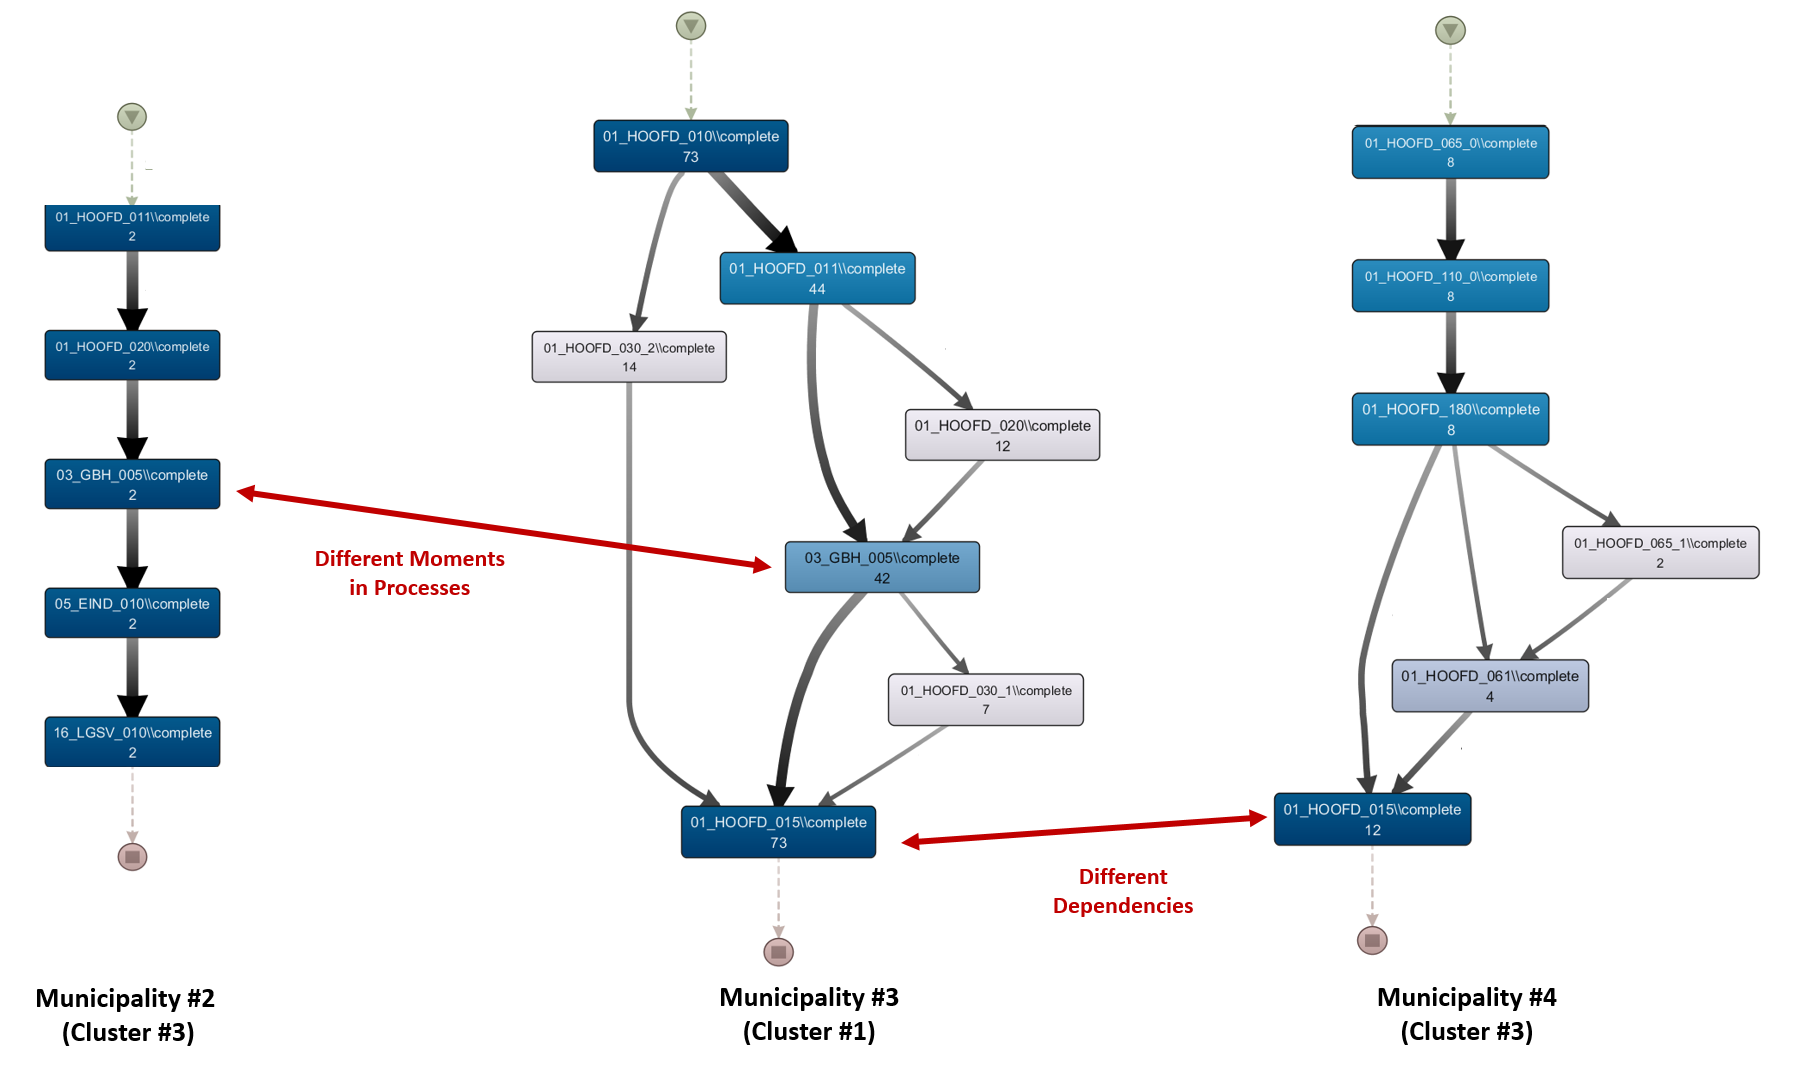
\includegraphics[width=\textwidth]{5_results_discussions/coselog-wabo/recommendation-visualization-mun-3}
			\caption{Visualization of example recommendation for Environmental Permit Application Process dataset (Municipality \#3)}
		  \label{fig:coselog-wabo-recommendation-visualization-mun-3}
		\end{figure} 

\end{itemize} % end of discussions